\input{preamble.tex}

\title{Лабораторная работа № 6. \\ Адресация IPv4 и IPv6. Двойной стек }
\author{Данила Стариков \\ НПИбд-02-22}
\institute{Российский университет дружбы народов имени Патриса Лумумбы}
\date{2025}

\begin{document}

\frame{\titlepage}

\begin{frame}
\frametitle{Цель работы}
\begin{itemize}
    \item Изучение принципов распределения и настройки адресного пространства на устройствах сети.
\end{itemize}
\end{frame}

\begin{frame}
\frametitle{Настройка двойного стека адресации IPv4 и IPv6 в локальной сети}
    \centering
    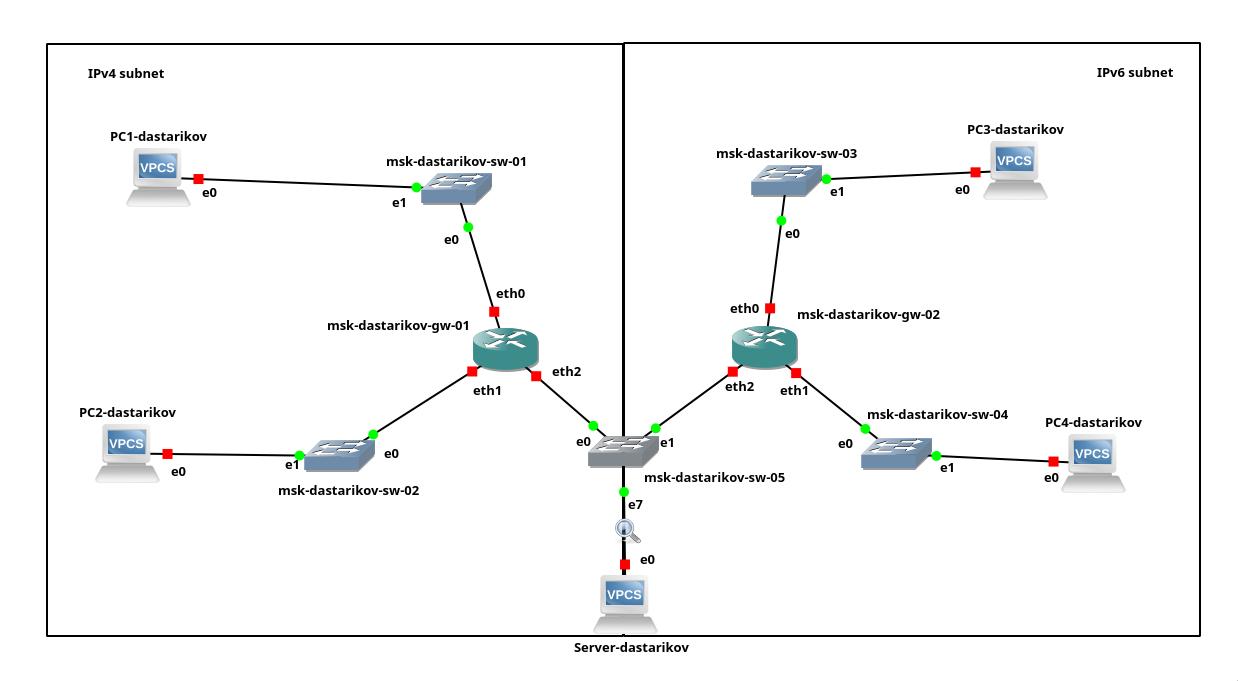
\includegraphics[width=\textwidth]{../images/image28.png}
    \captionof{figure}{Топология сети.}
\end{frame}


\begin{frame}
\frametitle{Настройка двойного стека адресации IPv4 и IPv6 в локальной сети}
\begin{table}[]
  \centering
  \caption{Таблица адресации}
  \label{tab1}
\footnotesize
\begin{tabular}{|llll|}
\hline
\multicolumn{1}{|l|}{Устройство} & \multicolumn{1}{l|}{Интерфейс} & \multicolumn{1}{l|}{IPv4-адрес} & Шлюз по умолчанию \\ \hline
gw-01                            & eth0                           & 172.16.20.1/25                  &                   \\
gw-01                            & eth1                           & 172.16.20.129/25                &                   \\
gw-01                            & eth2                           & 64.100.1.1/24                   &                   \\ \hline
PC1                              & NIC                            & 172.16.20.10/25                 & 172.16.20.1       \\
PC2                              & NIC                            & 172.16.20.138/25                & 172.16.20.129     \\ \hline
gw-02                            & eth0                           & 2001:db8:c0de:12::1/64          &                   \\
gw-02                            & eth1                           & 2001:db8:c0de:13::1/64          &                   \\
gw-02                            & eth2                           & 2001:db8:c0de:11::1/64          &                   \\ \hline
PC3                              & NIC                            & 2001:db8:c0de:12::a/64          & gw-02             \\
PC4                              & NIC                            & 2001:db8:c0de:13::a/64          & gw-02             \\ \hline
Server                           & NIC                            & 64.100.1.10/24                  & 64.100.1.1        \\
Server                           & NIC                            & 2001:db8:c0de:11::a/64          & gw-02             \\ \hline
\end{tabular}
\end{table}
\end{frame}

\begin{frame}
\frametitle{Настройка двойного стека адресации IPv4 и IPv6 в локальной сети}
    \centering
    
\includegraphics[width=\textwidth]{../images/image01.png}
    \captionof{figure}{Настройка IP-адреса на PC1.}
\end{frame}

\begin{frame}
\frametitle{Настройка двойного стека адресации IPv4 и IPv6 в локальной сети}
    \centering
    
\includegraphics[width=\textwidth]{../images/image02.png}
    \captionof{figure}{Настройка IP-адреса на PC2.}
\end{frame}

\begin{frame}
\frametitle{Настройка двойного стека адресации IPv4 и IPv6 в локальной сети}
    \centering
    
\includegraphics[width=\textwidth]{../images/image03.png}
    \captionof{figure}{Настройка IP-адреса на Server.}
\end{frame}

\begin{frame}
\frametitle{Настройка двойного стека адресации IPv4 и IPv6 в локальной сети}
    \centering
    
\includegraphics[width=0.6\textwidth]{../images/image04.png}
    \captionof{figure}{Просмотр конфигурации IPv4 и IPv6 на PC1.}
\end{frame}

\begin{frame}
\frametitle{Настройка двойного стека адресации IPv4 и IPv6 в локальной сети}
    \centering
    
\includegraphics[width=0.5\textwidth]{../images/image05.png}
    \captionof{figure}{Просмотр конфигурации IPv4 и IPv6 на PC2.}
\end{frame}

\begin{frame}
\frametitle{Настройка двойного стека адресации IPv4 и IPv6 в локальной сети}
    \centering
    
\includegraphics[width=\textwidth]{../images/image07.png}
    \captionof{figure}{Настройка IP-адреса на маршрутизаторе \texttt{gw-01}.}
\end{frame}

\begin{frame}
\frametitle{Настройка двойного стека адресации IPv4 и IPv6 в локальной сети}
    \centering
    
\includegraphics[width=0.5\textwidth]{../images/image09.png}
    \captionof{figure}{Просмотр конфигурации на маршрутизаторе \texttt{gw-01}.}
\end{frame}

\begin{frame}
\frametitle{Настройка двойного стека адресации IPv4 и IPv6 в локальной сети}
    \centering
    
\includegraphics[width=\textwidth]{../images/image11.png}
    \captionof{figure}{Проверка подключения между узлами PC1, PC2 и сервером сети.} 
\end{frame}

\begin{frame}
\frametitle{Настройка двойного стека адресации IPv4 и IPv6 в локальной сети}
    \centering
    
\includegraphics[width=\textwidth]{../images/image12.png}
    \captionof{figure}{Настройка IP-адреса на PC3.}
\end{frame}

\begin{frame}
\frametitle{Настройка двойного стека адресации IPv4 и IPv6 в локальной сети}
    \centering
    
\includegraphics[width=\textwidth]{../images/image13.png}
    \captionof{figure}{Настройка IP-адреса на PC4.}
\end{frame}

\begin{frame}
\frametitle{Настройка двойного стека адресации IPv4 и IPv6 в локальной сети}
    \centering
    
\includegraphics[width=\textwidth]{../images/image14.png}
    \captionof{figure}{Настройка IPv6-адреса на Server.}
\end{frame}

\begin{frame}
\frametitle{Настройка двойного стека адресации IPv4 и IPv6 в локальной сети}
    \centering
    
\includegraphics[width=0.6\textwidth]{../images/image15.png}
    \captionof{figure}{Просмотр конфигурации Server.}
\end{frame}

\begin{frame}
\frametitle{Настройка двойного стека адресации IPv4 и IPv6 в локальной сети}
    \centering
    
\includegraphics[width=0.6\textwidth]{../images/image16.png}
    \captionof{figure}{Просмотр конфигурации PC3.}
\end{frame}

\begin{frame}
\frametitle{Настройка двойного стека адресации IPv4 и IPv6 в локальной сети}
    \centering
    
\includegraphics[width=0.7\textwidth]{../images/image17.png}
    \captionof{figure}{Настройка имени устройства.}
\end{frame}

\begin{frame}
\frametitle{Настройка двойного стека адресации IPv4 и IPv6 в локальной сети}
    \centering
    
\includegraphics[width=0.4\textwidth]{../images/image18.png}
    \captionof{figure}{Конфигурация машрутизатора \texttt{gw-02}.}
\end{frame}

\begin{frame}
\frametitle{Настройка двойного стека адресации IPv4 и IPv6 в локальной сети}
    \centering
    
\includegraphics[width=0.7\textwidth]{../images/image19.png}
    \captionof{figure}{Проверка подключения узла PC3 к узлам PC4 и серверу.}
\end{frame}

\begin{frame}
\frametitle{Настройка двойного стека адресации IPv4 и IPv6 в локальной сети}
    \centering
    
\includegraphics[width=0.7\textwidth]{../images/image20.png}
    \captionof{figure}{Проверка подключения узла PC4 к узлам PC3 и серверу.}
\end{frame}

\begin{frame}
\frametitle{Настройка двойного стека адресации IPv4 и IPv6 в локальной сети}
    \centering
    
\includegraphics[width=\textwidth]{../images/image21.png}
    \captionof{figure}{Попытка подключения к узлам PC3 и PC4 с PC1.}
\end{frame}

\begin{frame}
\frametitle{Настройка двойного стека адресации IPv4 и IPv6 в локальной сети}
    \centering
    
\includegraphics[width=\textwidth]{../images/image22.png}
    \captionof{figure}{Попытка подключения к узлам PC3 и PC4 с PC2.}
\end{frame}

\begin{frame}
\frametitle{Настройка двойного стека адресации IPv4 и IPv6 в локальной сети}
    \centering
    
\includegraphics[width=\textwidth]{../images/image23.png}
    \captionof{figure}{Попытка подключения к узлам PC1 и PC1 с PC3.}
\end{frame}

\begin{frame}
\frametitle{Настройка двойного стека адресации IPv4 и IPv6 в локальной сети}
    \centering
    
\includegraphics[width=\textwidth]{../images/image24.png}
    \captionof{figure}{Попытка подключения к узлам PC1 и PC2 с PC4.}
\end{frame}


\begin{frame}
\frametitle{Настройка двойного стека адресации IPv4 и IPv6 в локальной сети}
    \centering
    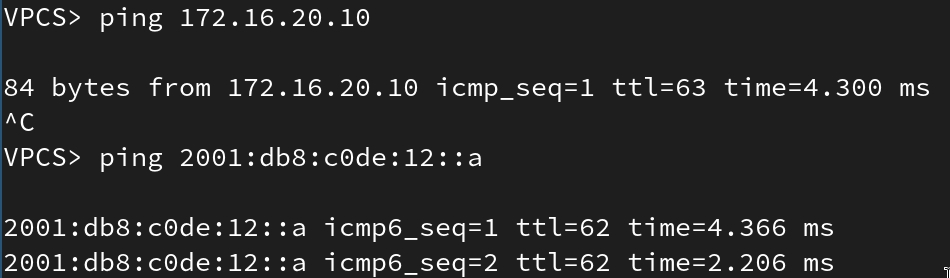
\includegraphics[width=\textwidth]{../images/image26.png}
    \captionof{figure}{Отправка эхо-запроса с сервера к PC1.}
\end{frame}

\begin{frame}
\frametitle{Настройка двойного стека адресации IPv4 и IPv6 в локальной сети}
    \centering
    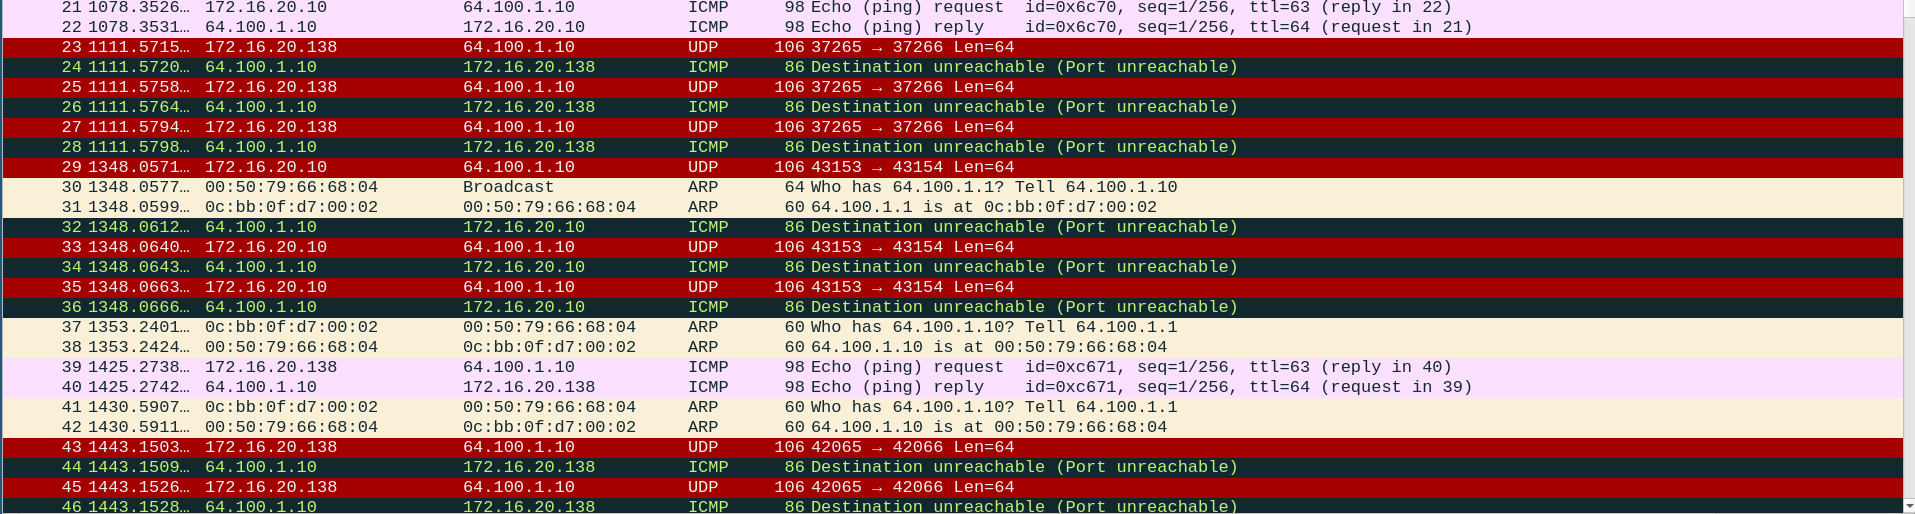
\includegraphics[width=\textwidth]{../images/image27.png}
    \captionof{figure}{Просмотр перехваченных пакетов.}
\end{frame}


\begin{frame}
\frametitle{Задание для самостоятельного выполнения}
    \centering
    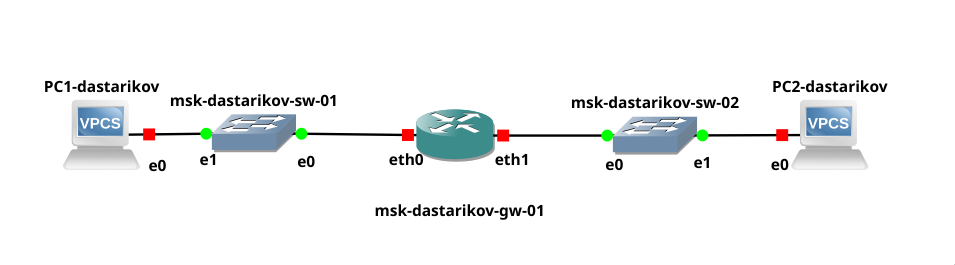
\includegraphics[width=\textwidth]{../images/image37.png}
    \captionof{figure}{Топология сети.}
\end{frame}

\begin{frame}
\frametitle{Задание для самостоятельного выполнения}

\begin{table}[]
\centering
\caption{Таблица адресации}
\label{tab2}
\tiny
\begin{tabular}{|l|l|l|l|l|}
\hline
Подсеть & Устройство           & Интерфейс & IPv4          & IPv6               \\ \hline
1         & PC1-dastarikov       & -         & 10.10.1.98/27 & 2001:db8:1:1::2/64 \\ \hline
2         & PC2-dastarikov       & -         & 10.10.1.18/28 & 2001:db8:1:4::2/64 \\ \hline
1         & msk-dastarikov-gw-01 & eth0      & 10.10.1.97/27 & 2001:db8:1:1::1/64 \\ \hline
2         & Msk-dastarikov-gw-01 & eth1      & 10.10.1.17/28 & 2001:db8:1:4::1/64 \\ \hline
\end{tabular}
\end{table}
\end{frame}

\begin{frame}
\frametitle{Задание для самостоятельного выполнения}
    \centering
    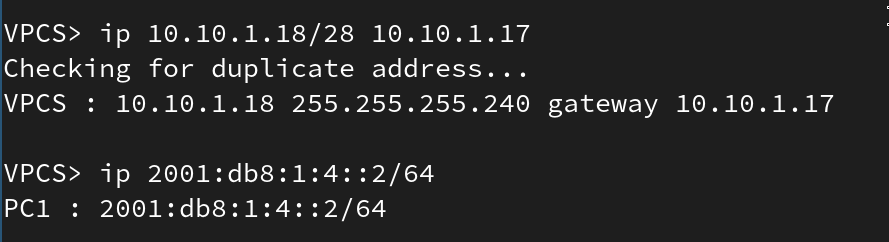
\includegraphics[width=\textwidth]{../images/image29.png}
    \captionof{figure}{Задание IP-адреса для PC1.}
\end{frame}

\begin{frame}
\frametitle{Задание для самостоятельного выполнения}
    \centering
    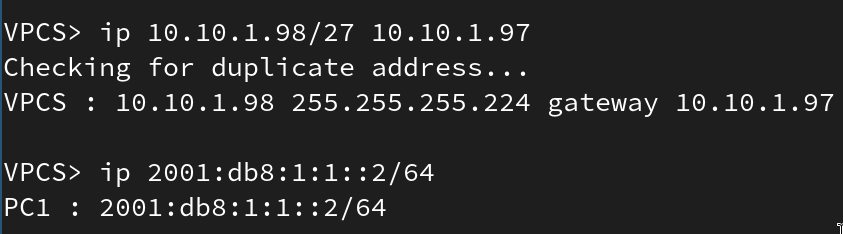
\includegraphics[width=\textwidth]{../images/image30.png}
    \captionof{figure}{Задание IP-адреса для PC2.}
\end{frame}

\begin{frame}
\frametitle{Задание для самостоятельного выполнения}
    \centering
    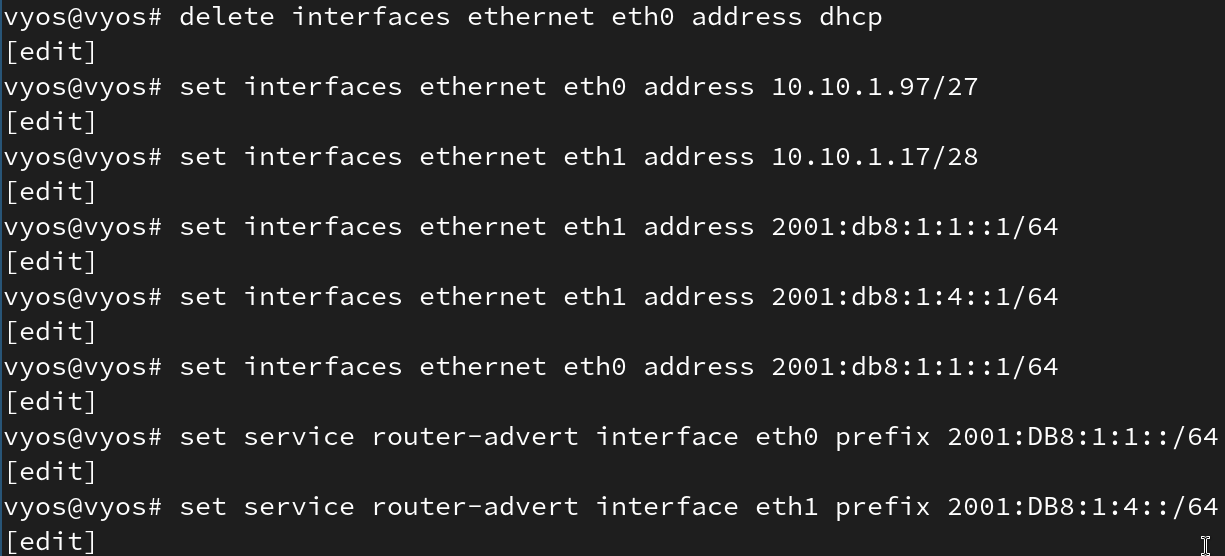
\includegraphics[width=\textwidth]{../images/image31.png}
    \captionof{figure}{Конфигурирование интерфейсов маршрутизатора.}
\end{frame}

\begin{frame}
\frametitle{Задание для самостоятельного выполнения}
    \centering
    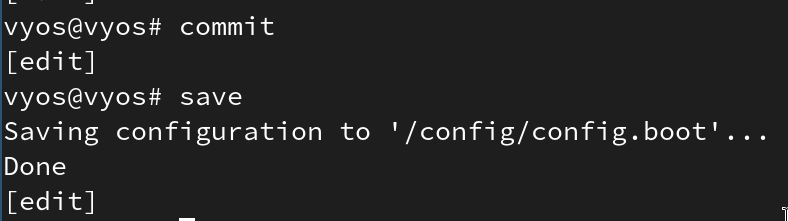
\includegraphics[width=\textwidth]{../images/image33.png}
    \captionof{figure}{Сохранение настроек.}
\end{frame}

\begin{frame}
\frametitle{Задание для самостоятельного выполнения}
    \centering
    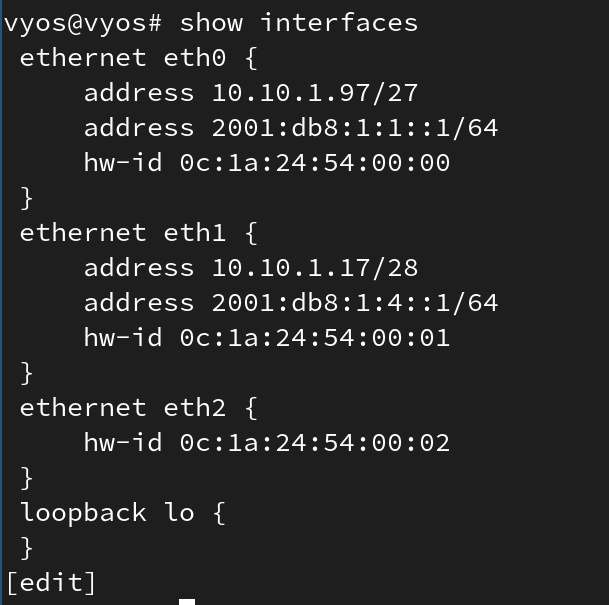
\includegraphics[width=0.7\textwidth]{../images/image34.png}
    \captionof{figure}{Просмотр текущей конфигурации интерфейсов маршрутизатора.}
\end{frame}

\begin{frame}
\frametitle{Задание для самостоятельного выполнения}
    \centering
    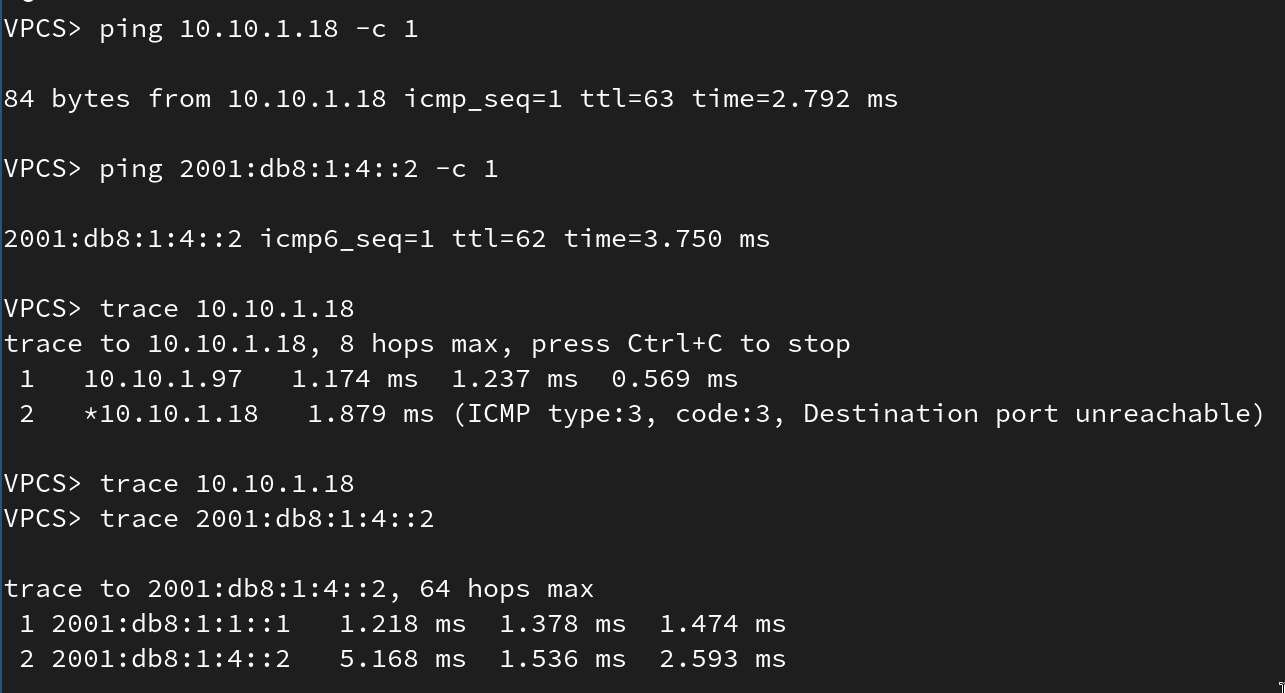
\includegraphics[width=\textwidth]{../images/image35.png}
    \captionof{figure}{Отправка эхо-запроса от PC1 к PC2.}
\end{frame}

\begin{frame}
\frametitle{Задание для самостоятельного выполнения}
    \centering
    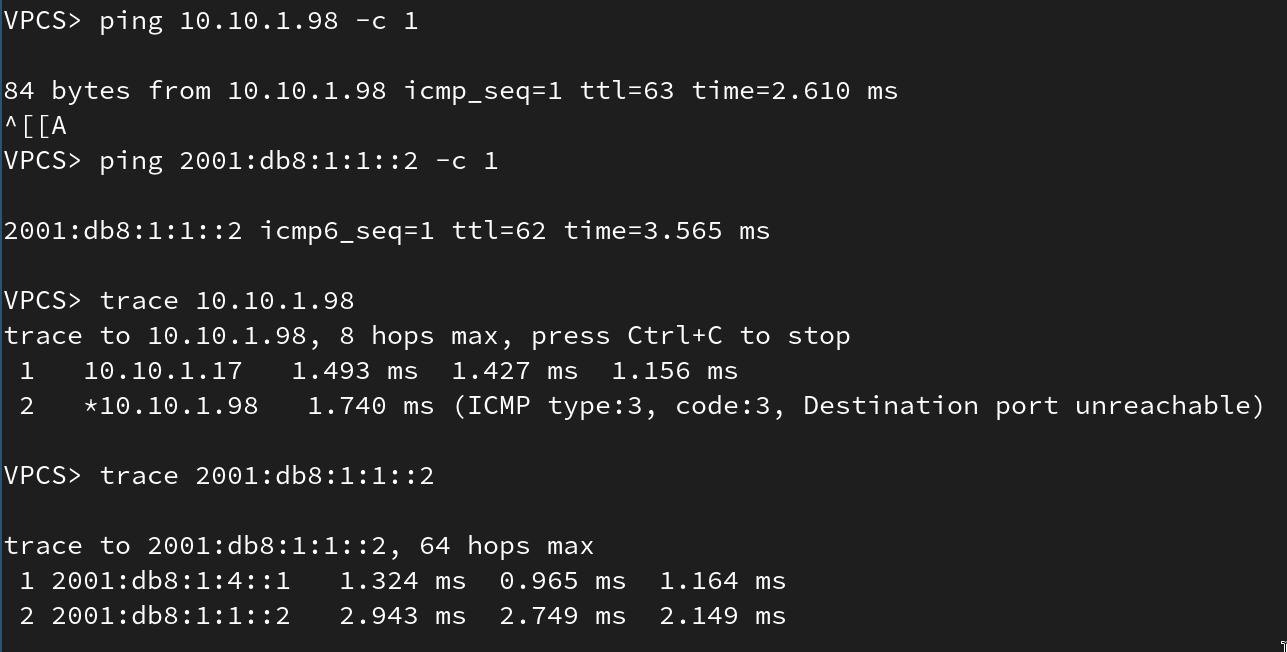
\includegraphics[width=\textwidth]{../images/image36.png}
    \captionof{figure}{Отправка эхо-запроса от PC2 к PC1.}
\end{frame}

\begin{frame}
\frametitle{Выводы}
\begin{itemize}
    \item В результате выполнения лабораторной работы изучили принципы распределения и настройки адресного пространства на устройствах сети.
\end{itemize}
\end{frame}
\end{document}
